\section{Detección de elementos del juego}
\label{sec:deteccion-elementos-juego}

La primera fase del pipeline consiste en detectar, fotograma a fotograma, los elementos relevantes del partido. Para esta tarea se empleó YOLOv11m, donde la letra \texttt{m} hace referencia a la variante \textit{medium}, elegida por ofrecer un compromiso razonable entre precisión y coste computacional.

Como punto de partida se utilizó el modelo base, es decir, el modelo preentrenado sin adaptación específica al dominio futbolístico. Al aplicarlo directamente sobre vídeo de fútbol, el modelo detecta jugadores, árbitros y porteros principalmente como instancias de la clase \texttt{person}, mientras que el balón puede aparecer como \texttt{sports ball}. Esto puede observarse en la \hyperref[fig:raw-detection-yolo11m]{Figura~\ref*{fig:raw-detection-yolo11m}}. Esta salida inicial permite comprobar que el detector reconoce objetos relevantes en la escena, pero no proporciona todavía la separación semántica necesaria para el proyecto, ya que agrupa todos los participantes humanos en una misma clase.

\begin{figure}[H]
    \centering
    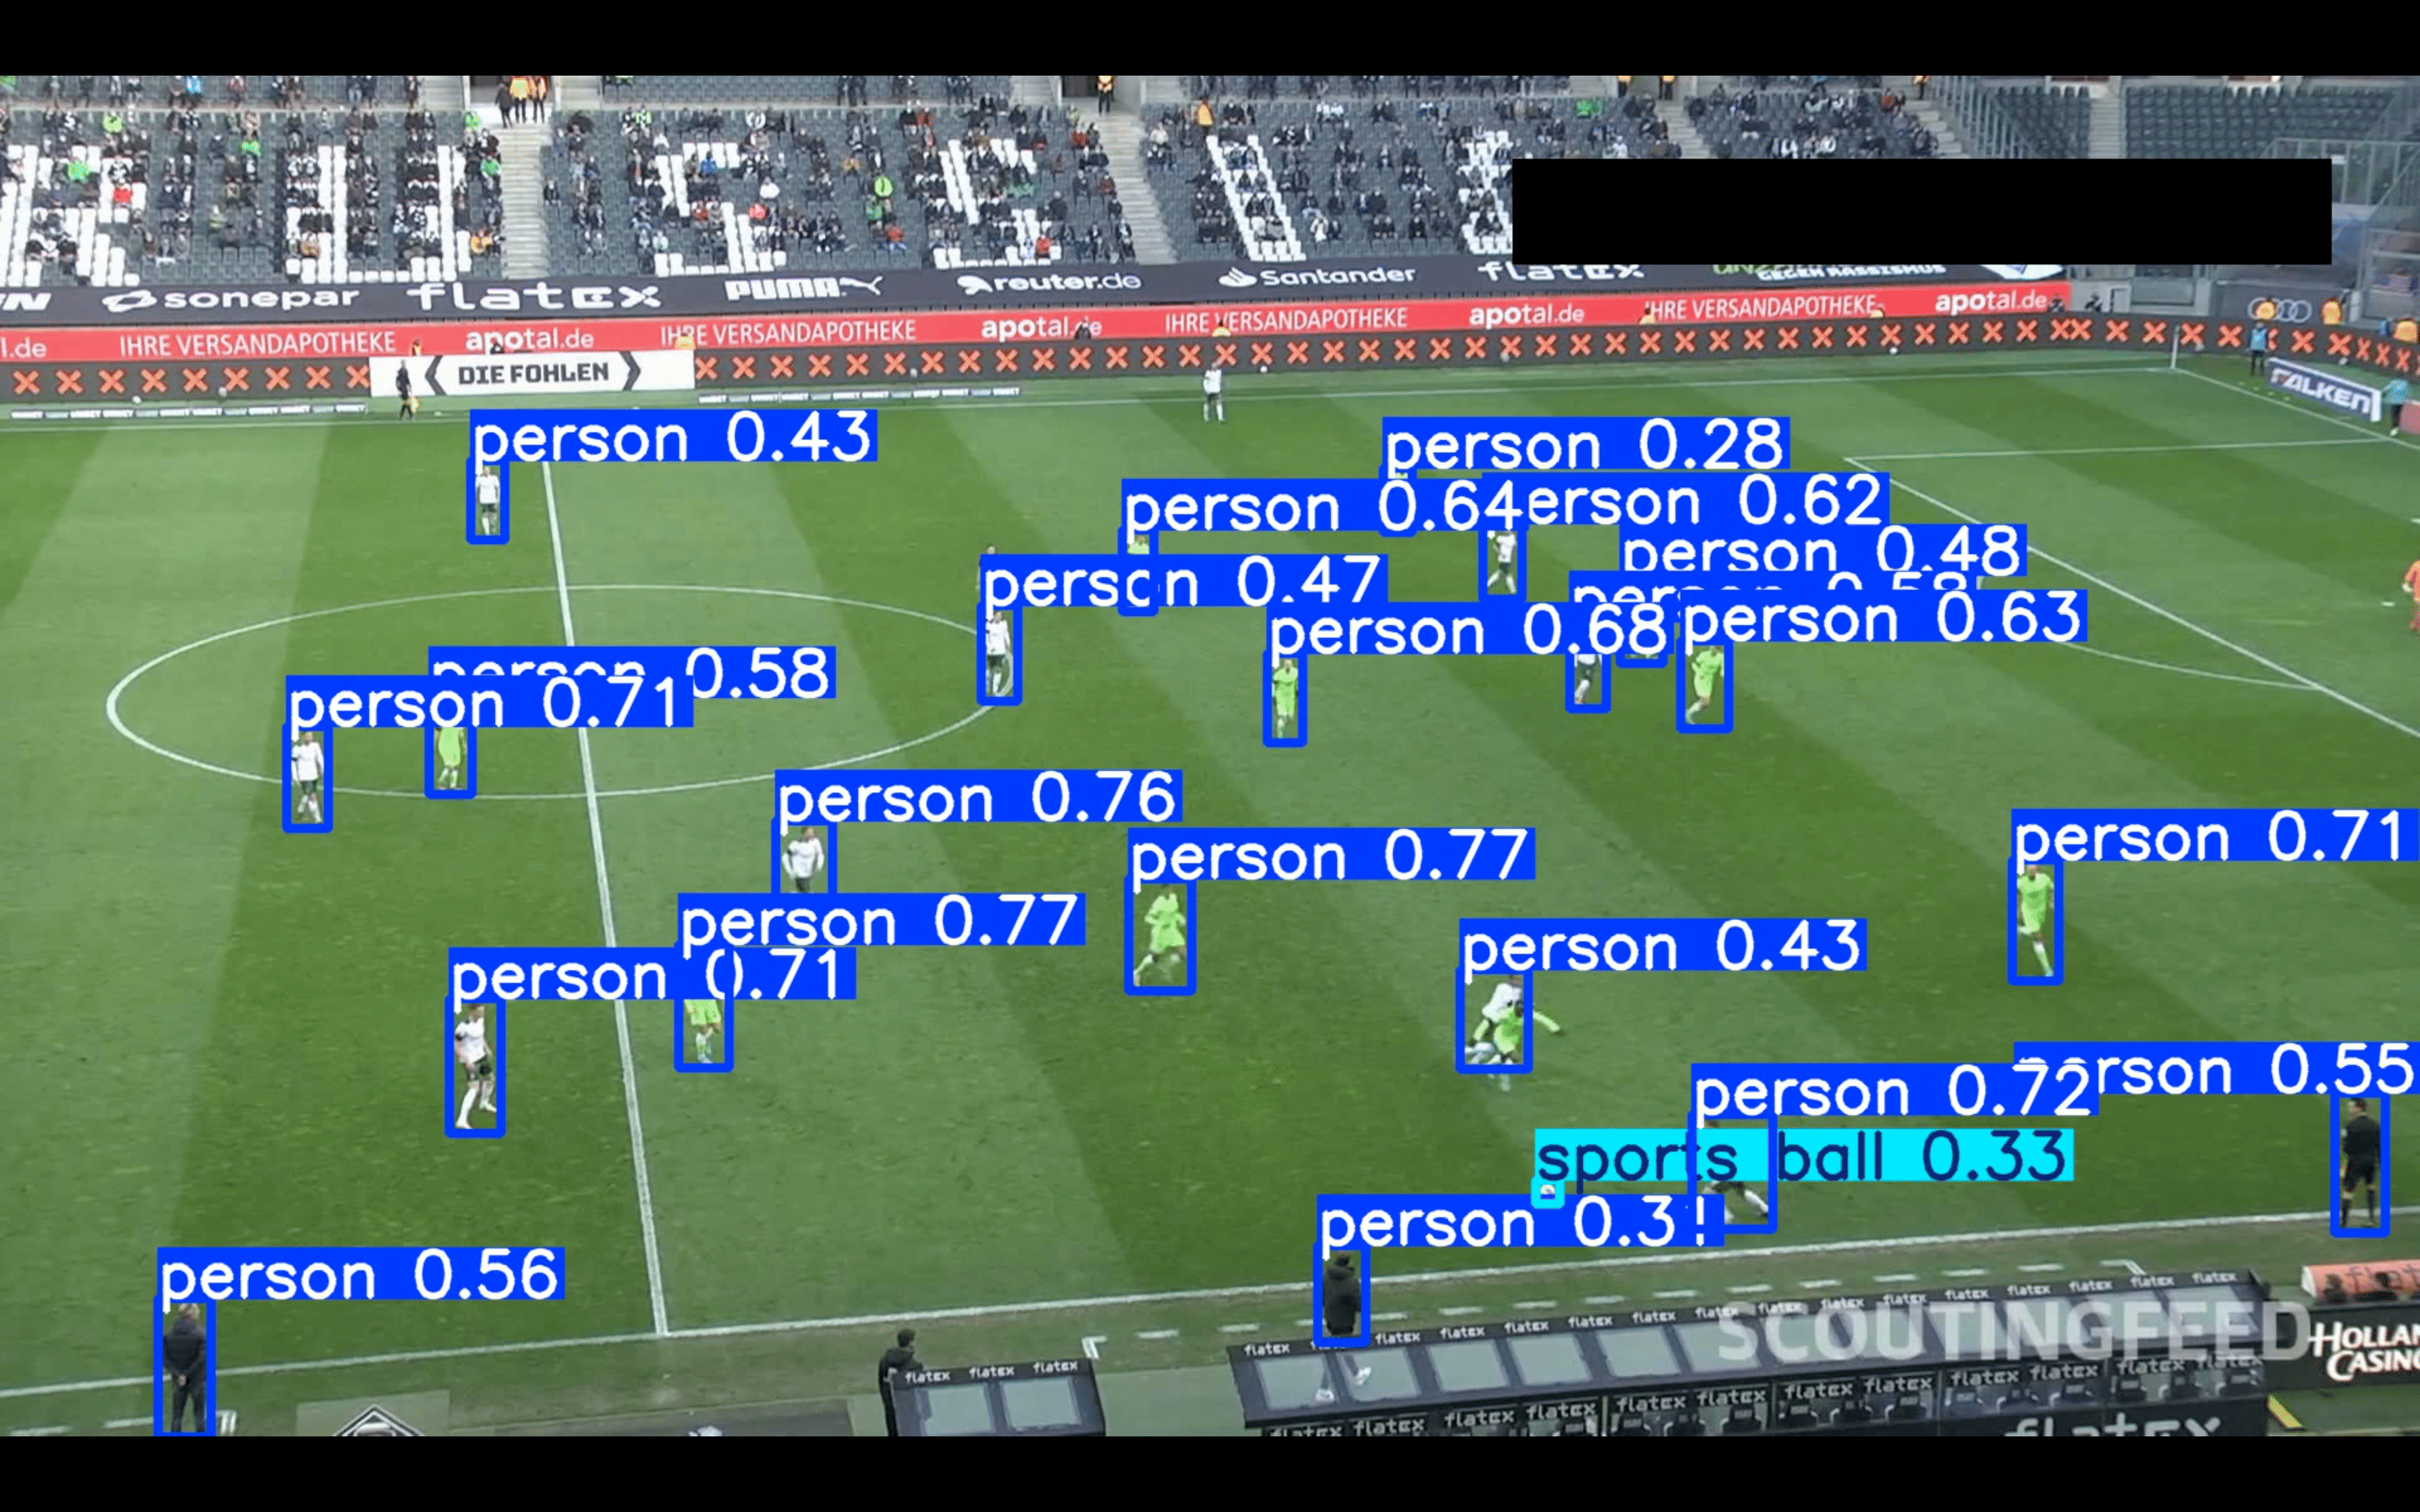
\includegraphics[width=0.9\linewidth]{Imagenes/Propias/Raw_detection.png}
    \caption[Detección inicial con YOLOv11m]{Detección inicial realizada con YOLOv11m base sobre un frame del partido.}
    \label{fig:raw-detection-yolo11m}
\end{figure}

Para observar el comportamiento del modelo base se realizó una prueba exploratoria sobre un clip corto de 10 frames. YOLO proporciona para cada detección un valor de confianza (\textit{confidence}), que representa la seguridad estimada del modelo respecto a la clase predicha. Los resultados se muestran en la Tabla \ref{tab:yolo11mBaseFrame}.

\begin{table}[H]
	\centering
	\begin{tabular}{c|c|c|c|c}
		\textbf{Frame} & \textbf{Personas} & \textbf{Balón} & \textbf{Conf. media} & \textbf{Conf. max} \\
		\hline\hline
		1 & 22 & 0 & 0.5646 & 0.7637 \\
		2 & 22 & 0 & 0.5741 & 0.7864 \\
		3 & 22 & 0 & 0.5724 & 0.7894 \\
		4 & 23 & 1 & 0.5370 & 0.7900 \\
		5 & 23 & 1 & 0.5094 & 0.7775 \\
		6 & 23 & 0 & 0.5514 & 0.7846 \\
		7 & 23 & 0 & 0.5571 & 0.7727 \\
		8 & 21 & 1 & 0.5781 & 0.7730 \\
		9 & 20 & 1 & 0.6162 & 0.7941 \\
		10 & 19 & 1 & 0.5925 & 0.7862 \\
		\hline
	\end{tabular}
	\caption[Prueba exploratoria de detección con YOLOv11m]{Prueba exploratoria de detección con YOLOv11m base sobre un clip corto de 10 frames.}
	\label{tab:yolo11mBaseFrame}
\end{table}

Los resultados muestran que el modelo detecta de forma estable a las personas presentes en la escena, con entre 19 y 23 detecciones por frame. Sin embargo, la detección del balón resulta más irregular, ya que solo aparece en 5 de los 10 frames analizados.

Sin embargo, para este proyecto no basta con detectar personas genéricas: es necesario distinguir entre elementos futbolísticos concretos, como jugadores, árbitros, porteros y balón. Por este motivo se decidió adaptar el detector mediante \textit{fine-tuning}.

\subsection{Adaptación del detector mediante \textit{fine-tuning}}
Como el modelo YOLOv11m base no proporcionaba la separación semántica necesaria para el proyecto, se decidió adaptar el detector al dominio futbolístico mediante \textit{fine-tuning}. El objetivo era que el modelo no solo detectara personas genéricas, sino que distinguiera entre clases relevantes para el sistema, como jugadores, árbitros, porteros y balón.


\subsubsection{Conjuntos de datos utilizados}

Para esta adaptación se emplearon tres conjuntos de datos con funciones distintas dentro del proceso de entrenamiento. La \hyperref[tab:datasets-finetuning-yolo]{Tabla~\ref*{tab:datasets-finetuning-yolo}} resume su procedencia, clases anotadas, tamaño y uso dentro del proyecto.

\begin{table}[H]
\centering
\scriptsize
\renewcommand{\arraystretch}{1.25}
\begin{tabularx}{\textwidth}{
>{\raggedright\arraybackslash}p{2.4cm}
>{\raggedright\arraybackslash}X
>{\raggedright\arraybackslash}p{2.8cm}
>{\raggedright\arraybackslash}p{2.5cm}
>{\raggedright\arraybackslash}X
}
\toprule
\textbf{Dataset} & \textbf{Url} & \textbf{Clases} & \textbf{Tamaño / partición} & \textbf{Uso} \\
\midrule

Roboflow fútbol \label{} &
\href{https://universe.roboflow.com/yolo-atnlh/football-detection-wfhdh}{Roboflow - FootBall Detection Computer Vision Model} &
\texttt{ball}, \texttt{player}, \texttt{referee}, \texttt{goalkeeper} $\rightarrow$ \texttt{player}. &
Train/val/test: 612/38/13 &
Primer \textit{fine-tuning} supervisado con clases futbolísticas. \\

\midrule

Datos sintéticos &
\href{https://research.spiideo.com/login/main.html}{Spiideo SoccerNet SynLoc} &
\texttt{person} $\rightarrow$ \texttt{player}. &
Train/val/test: 42.554/6.777/9.309 &
Adaptación intermedia sintética al dominio futbolístico: césped, jugadores, variación de cámara, iluminación y desenfoque de movimiento.. \\

\midrule

DFL-Bundesliga &
\href{https://universe.roboflow.com/inkyu-sa-e0c78/dfl-bundesliga-soccer-football-gpqdy}{Roboflow - DFL-Bundesliga} &
\texttt{ball}, \texttt{player}, \texttt{referee}. &
Train/val/test: 19.068/2.434/2.455 &
Refinamiento final sobre datos reales más próximos al escenario objetivo. \\

\bottomrule
\end{tabularx}
\caption[Conjuntos de datos utilizados para el fine-tuning del detector]{
Conjuntos de datos utilizados durante la adaptación del detector YOLOv11m al dominio futbolístico.
}
\label{tab:datasets-finetuning-yolo}
\end{table}

\noindent\textit{Nota:} Para homogeneizar el entrenamiento entre fases, las clases se adaptaron al formato final del detector: \texttt{player}, \texttt{referee} y \texttt{ball}. En SoccerSynth-Detection, la clase original \texttt{person} se mapeó a \texttt{player}; las clases \texttt{referee} y \texttt{ball} se incluyeron en la definición de clases, aunque no tenían instancias anotadas en ese conjunto. En el dataset Roboflow fútbol, la clase \texttt{goalkeeper} se integró dentro de \texttt{player}.

\subsubsection{Estrategias de entrenamiento}

Se exploraron dos estrategias principales de adaptación. La primera consistió en entrenar YOLOv11m directamente sobre el pequeño dataset \textit{Roboflow fútbol} obtenido en Roboflow. Este dataset permitía introducir clases futbolísticas concretas, como \texttt{ball}, \texttt{player}, \texttt{referee} y \texttt{goalkeeper}, y servía como primer intento de especialización del modelo base. Además, el proyecto de Roboflow incluía un modelo de referencia con métricas publicadas de \textit{mAP@50} del 82.1\%, precisión del 96.7\% y recall del 75.2\%. Estas métricas no se interpretan como resultados propios ni como una evaluación del dataset, sino como un indicio inicial de que las anotaciones y la definición de clases podían ser útiles para adaptar el detector al dominio futbolístico.

La segunda estrategia consistió en un \textit{fine-tuning} secuencial. En primer lugar, el modelo se entrenó sobre SoccerSynth-Detection \citep{SoccerSynthDetection2025}, un conjunto sintético orientado a detección en fútbol. Esta fase tenía como objetivo adaptar el detector al dominio visual del fútbol, exponiéndolo a escenas con césped, jugadores, variaciones de cámara, iluminación y desenfoque de movimiento. Posteriormente, el modelo resultante se refinó sobre DFL-Bundesliga, un conjunto de imágenes reales con clases más próximas al problema final: \texttt{ball}, \texttt{player} y \texttt{referee}.

La motivación de esta estrategia secuencial era aprovechar primero la variabilidad controlada de los datos sintéticos y, después, ajustar el modelo sobre datos reales más cercanos al escenario de aplicación. De esta forma, se buscaba mejorar la capacidad de generalización del detector antes de integrarlo en el pipeline completo.

\subsubsection{Resultados del \textit{fine-tuning} secuencial} 

La \hyperref[fig:results_finetuning_compare]{Figura~\ref*{fig:results_finetuning_compare}} muestra las curvas de entrenamiento de las dos fases del \textit{fine-tuning} secuencial. En la fase sintética, las métricas convergen rápidamente y se estabilizan hacia la mitad del entrenamiento, alcanzando un mAP@50-95 final cercano a 0.80. En la fase DFL-Bundesliga, la mejora es más gradual y las métricas finales son menores, con un mAP@50-95 cercano a 0.63.

\begin{figure}[H]
\centering

\begin{minipage}{0.95\textwidth}
    \centering
    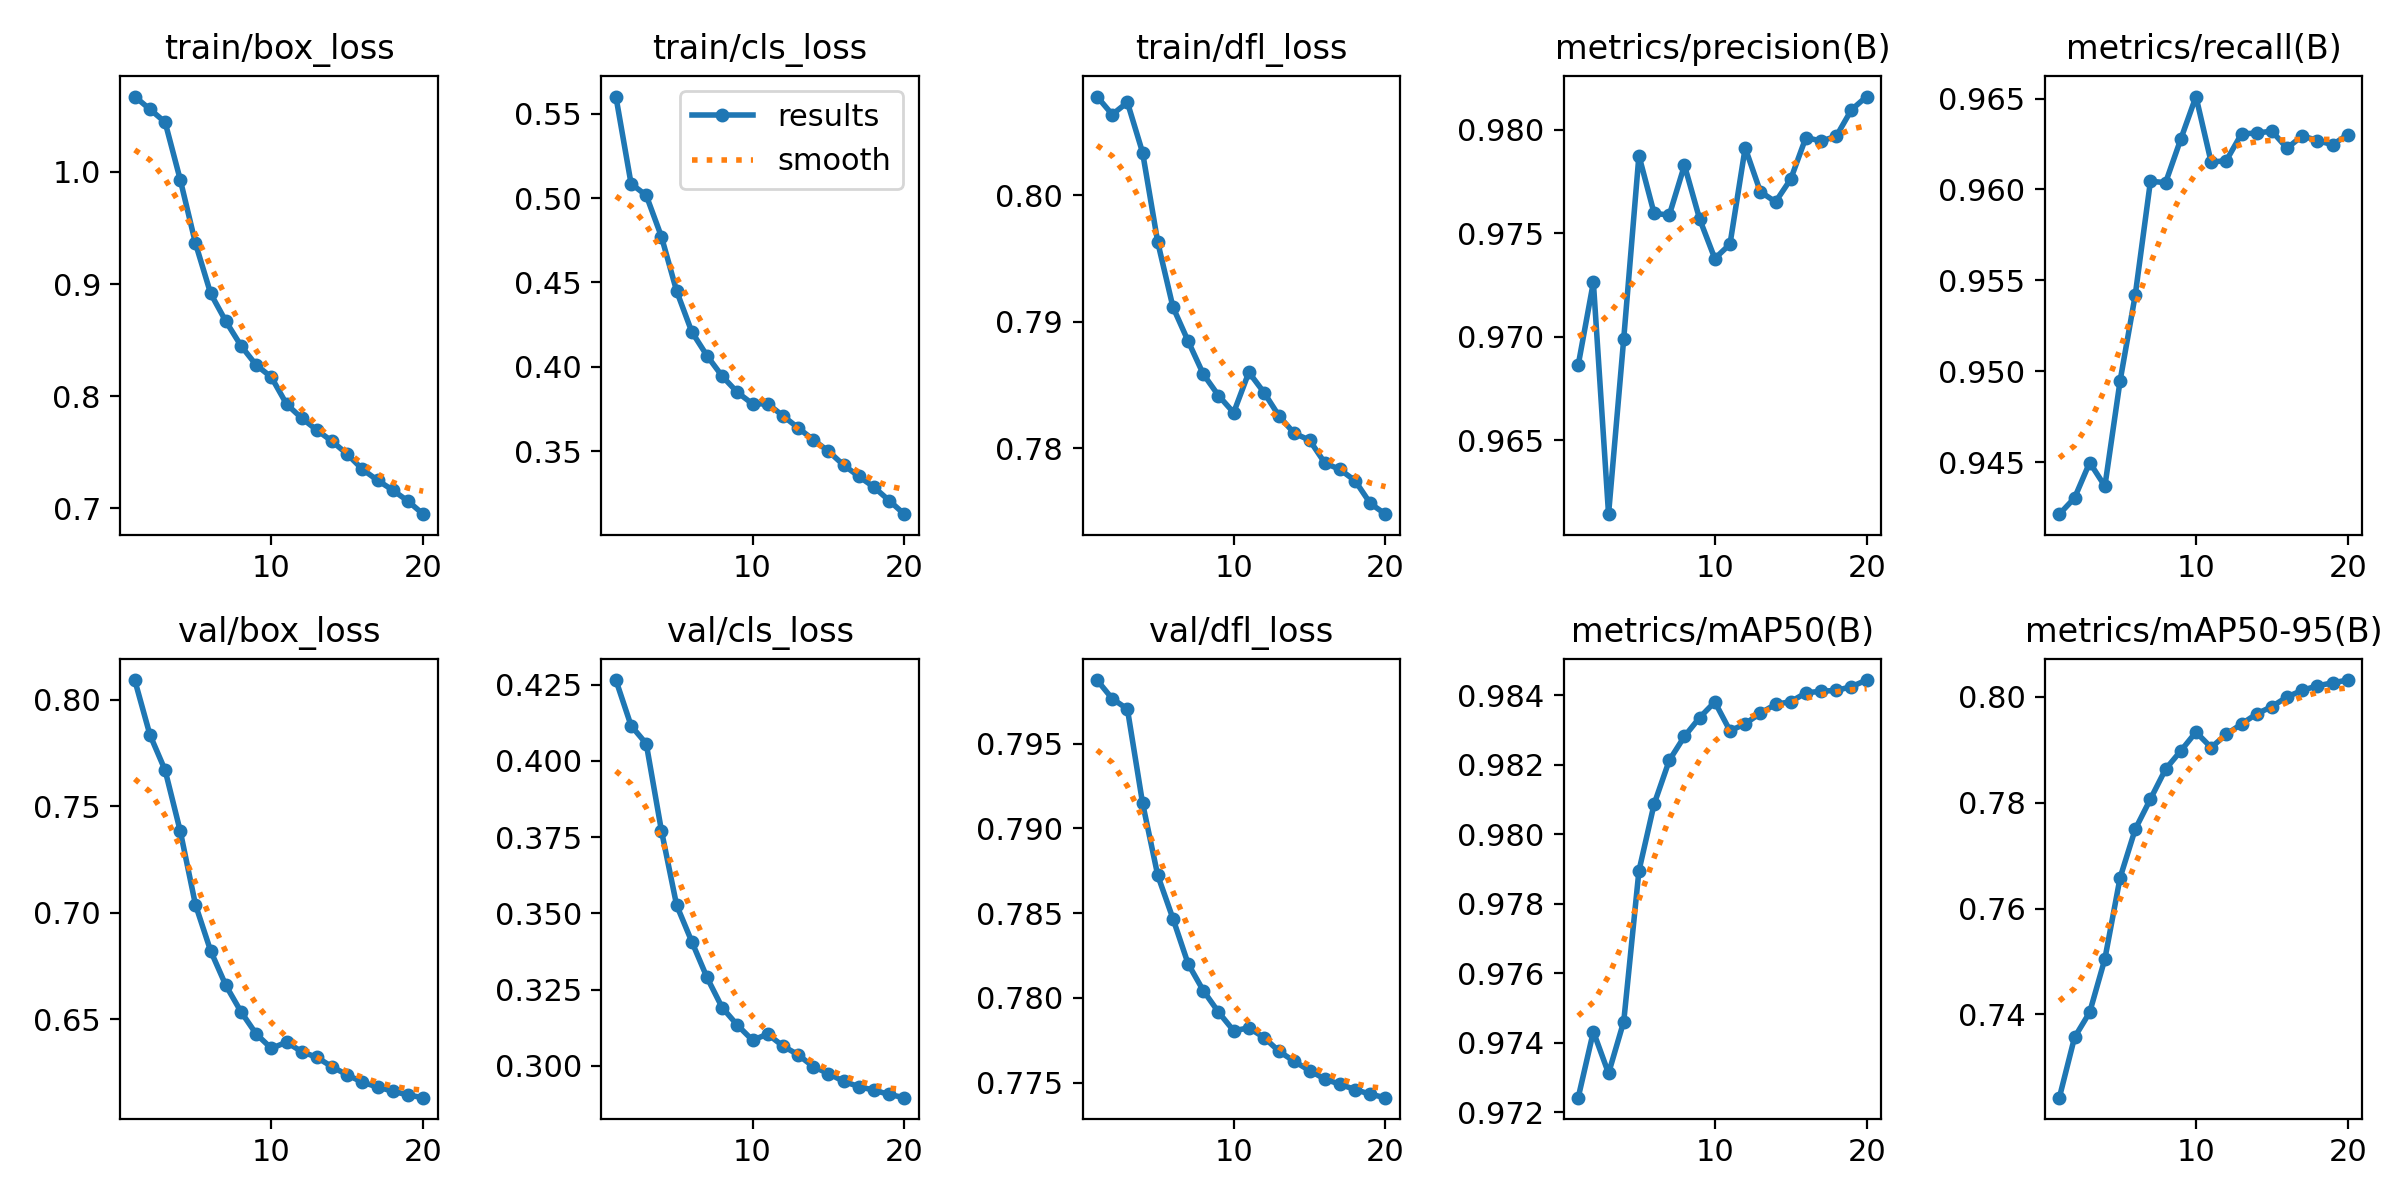
\includegraphics[width=\textwidth]{Imagenes/Propias/results_sinteticos.png}
    \small \textbf{(a)} Primera fase del \textit{fine-tuning} secuencial sobre SoccerSynth-Detection.
\end{minipage}

\vspace{0.4cm}

\begin{minipage}{0.95\textwidth}
    \centering
    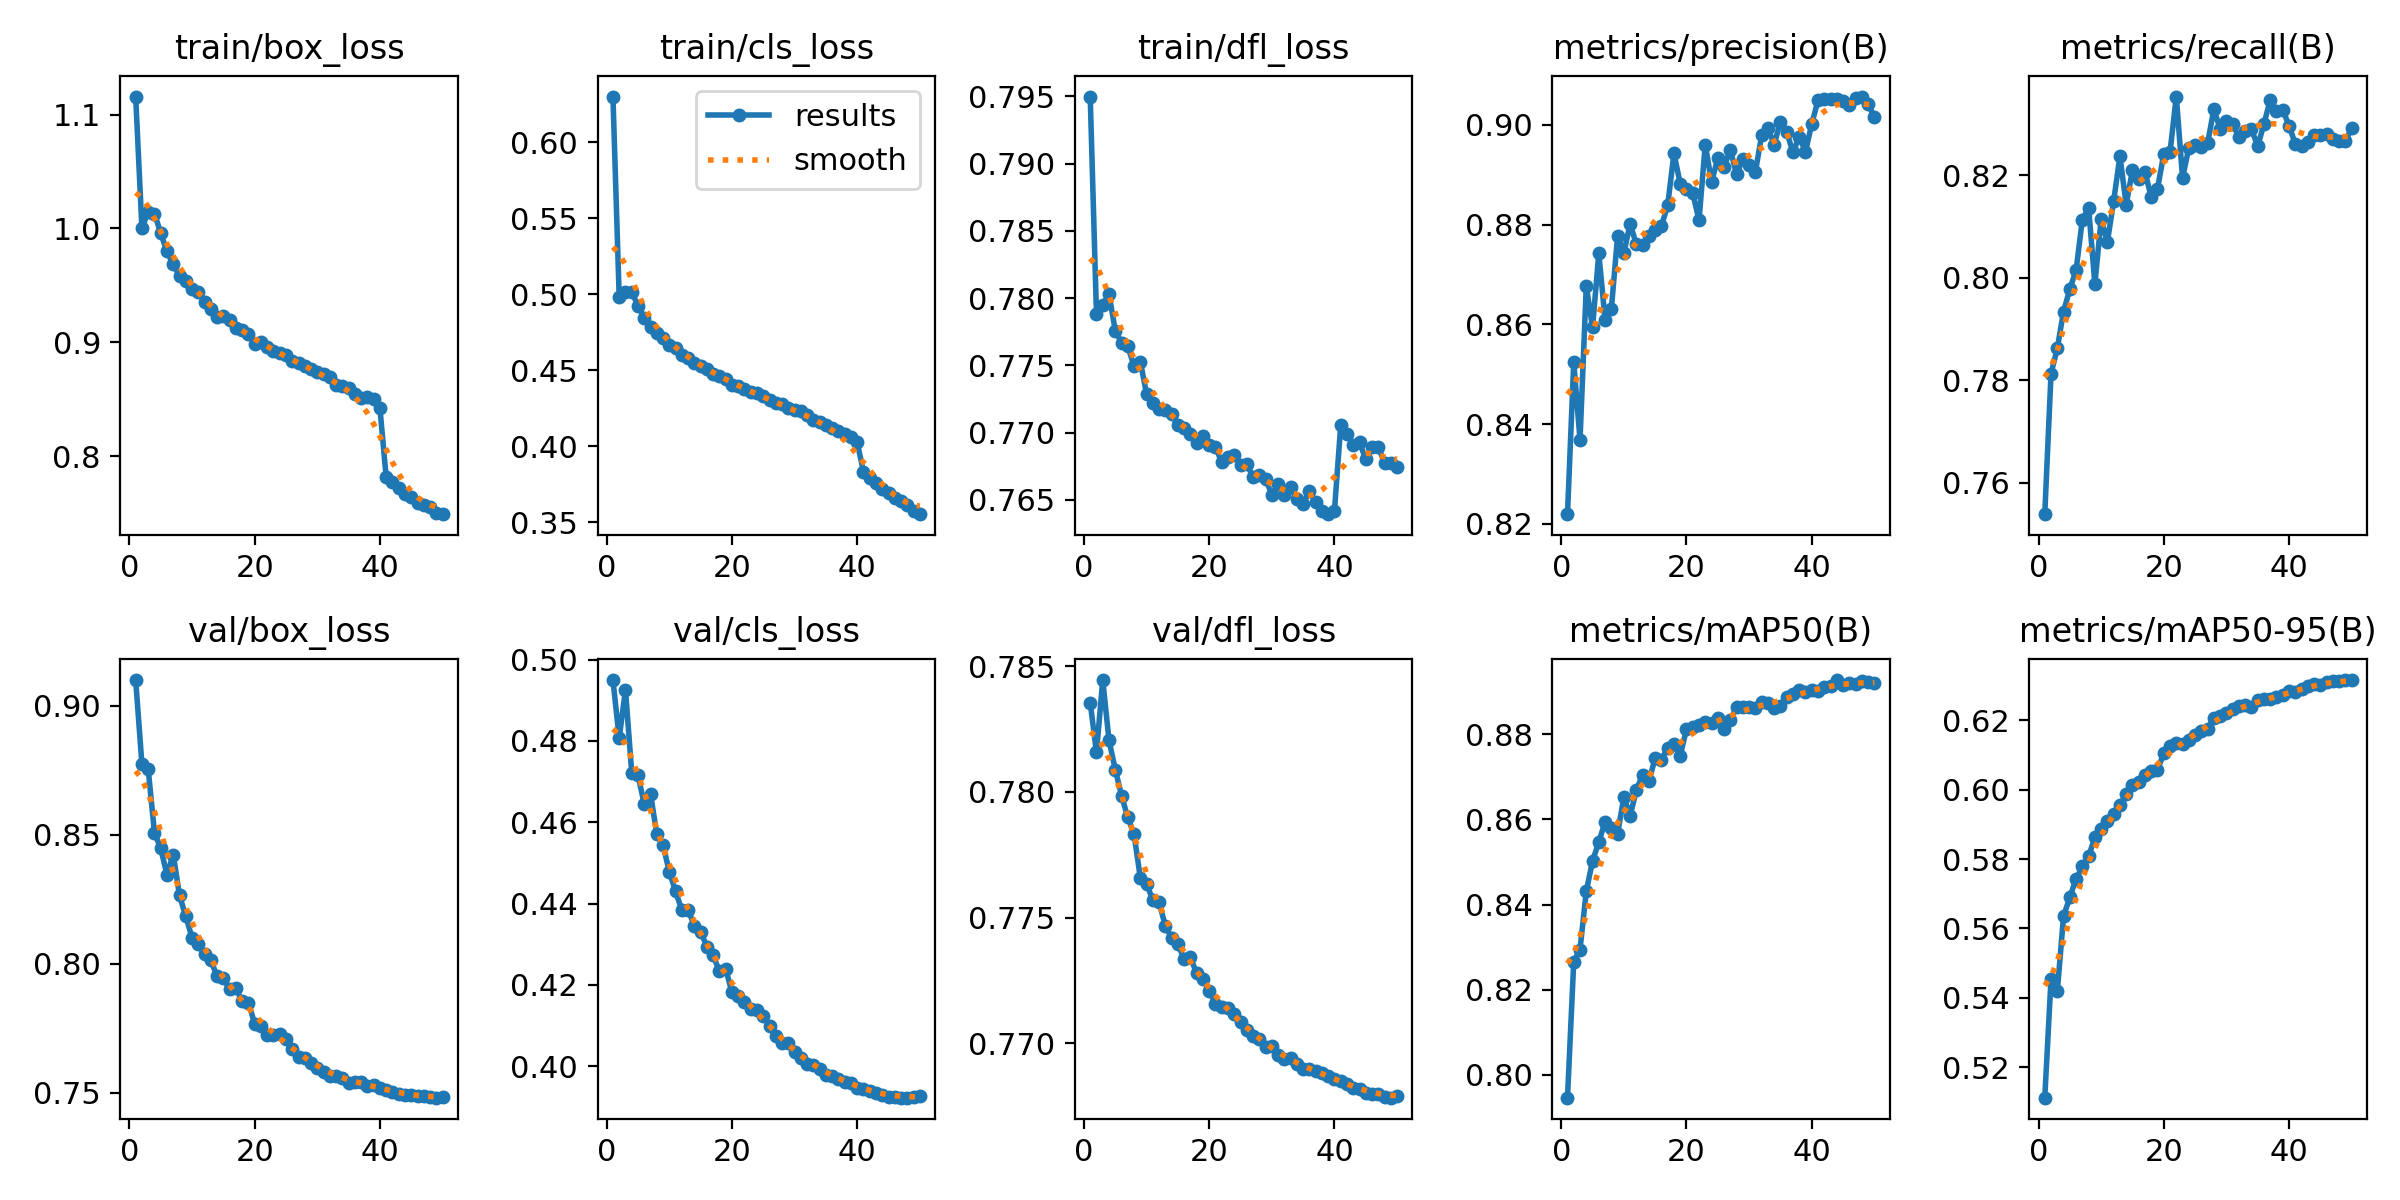
\includegraphics[width=\textwidth]{Imagenes/Propias/results_dfl.png}
    \small \textbf{(b)} Segunda fase del \textit{fine-tuning} secuencial sobre DFL-Bundesliga.
\end{minipage}

\caption[Curvas de entrenamiento del fine-tuning secuencial]{
Curvas de entrenamiento del proceso de \textit{fine-tuning} secuencial.
}
\label{fig:results_finetuning_compare}
\end{figure}

La \hyperref[tab:comparacion_modelos_finetuneados]{Tabla~\ref*{tab:comparacion_modelos_finetuneados}} resume las métricas finales de ambas fases, evaluadas sobre sus respectivos conjuntos de validación. Aunque las métricas de la fase sintética son superiores, no deben interpretarse como una comparación directa entre modelos equivalentes, ya que cada fase utiliza un conjunto de datos distinto. La primera fase sintética trabaja sobre una tarea más simple, homogénea y de una sola clase, mientras que la segunda introduce un dominio más realista y clases más específicas.

\begin{table}[H]
\centering
\scriptsize
\begin{tabular}{c|c|c|c|c|c|c|c}
\textbf{Fase} & \textbf{Ep.} & \textbf{Batch} & \textbf{Imgsz} & \textbf{Prec. final} & \textbf{Recall final} & \textbf{mAP@50} & \textbf{mAP@50-95} \\
\hline\hline
Datos sintéticos & 20 & 8 & 1280 & 0.9816 & 0.9630 & 0.9844 & 0.8032 \\
\hline
DFL-Bundesliga & 50 & 16 & 640 & 0.8911 & 0.8352 & 0.8909 & 0.6305 \\
\hline
\end{tabular}
\caption[Métricas finales del fine-tuning secuencial]{
Métricas finales de validación de las dos fases del \textit{fine-tuning} secuencial.
}
\label{tab:comparacion_modelos_finetuneados}
\end{table}

Para interpretar estas diferencias, la \hyperref[fig:datasets_summary]{Figura~\ref*{fig:datasets_summary}} compara la distribución de clases y las características espaciales de las cajas anotadas en los conjuntos utilizados durante el \textit{fine-tuning} secuencial.

\begin{figure}[H]
\centering

\begin{minipage}{0.55\textwidth}
    \centering
    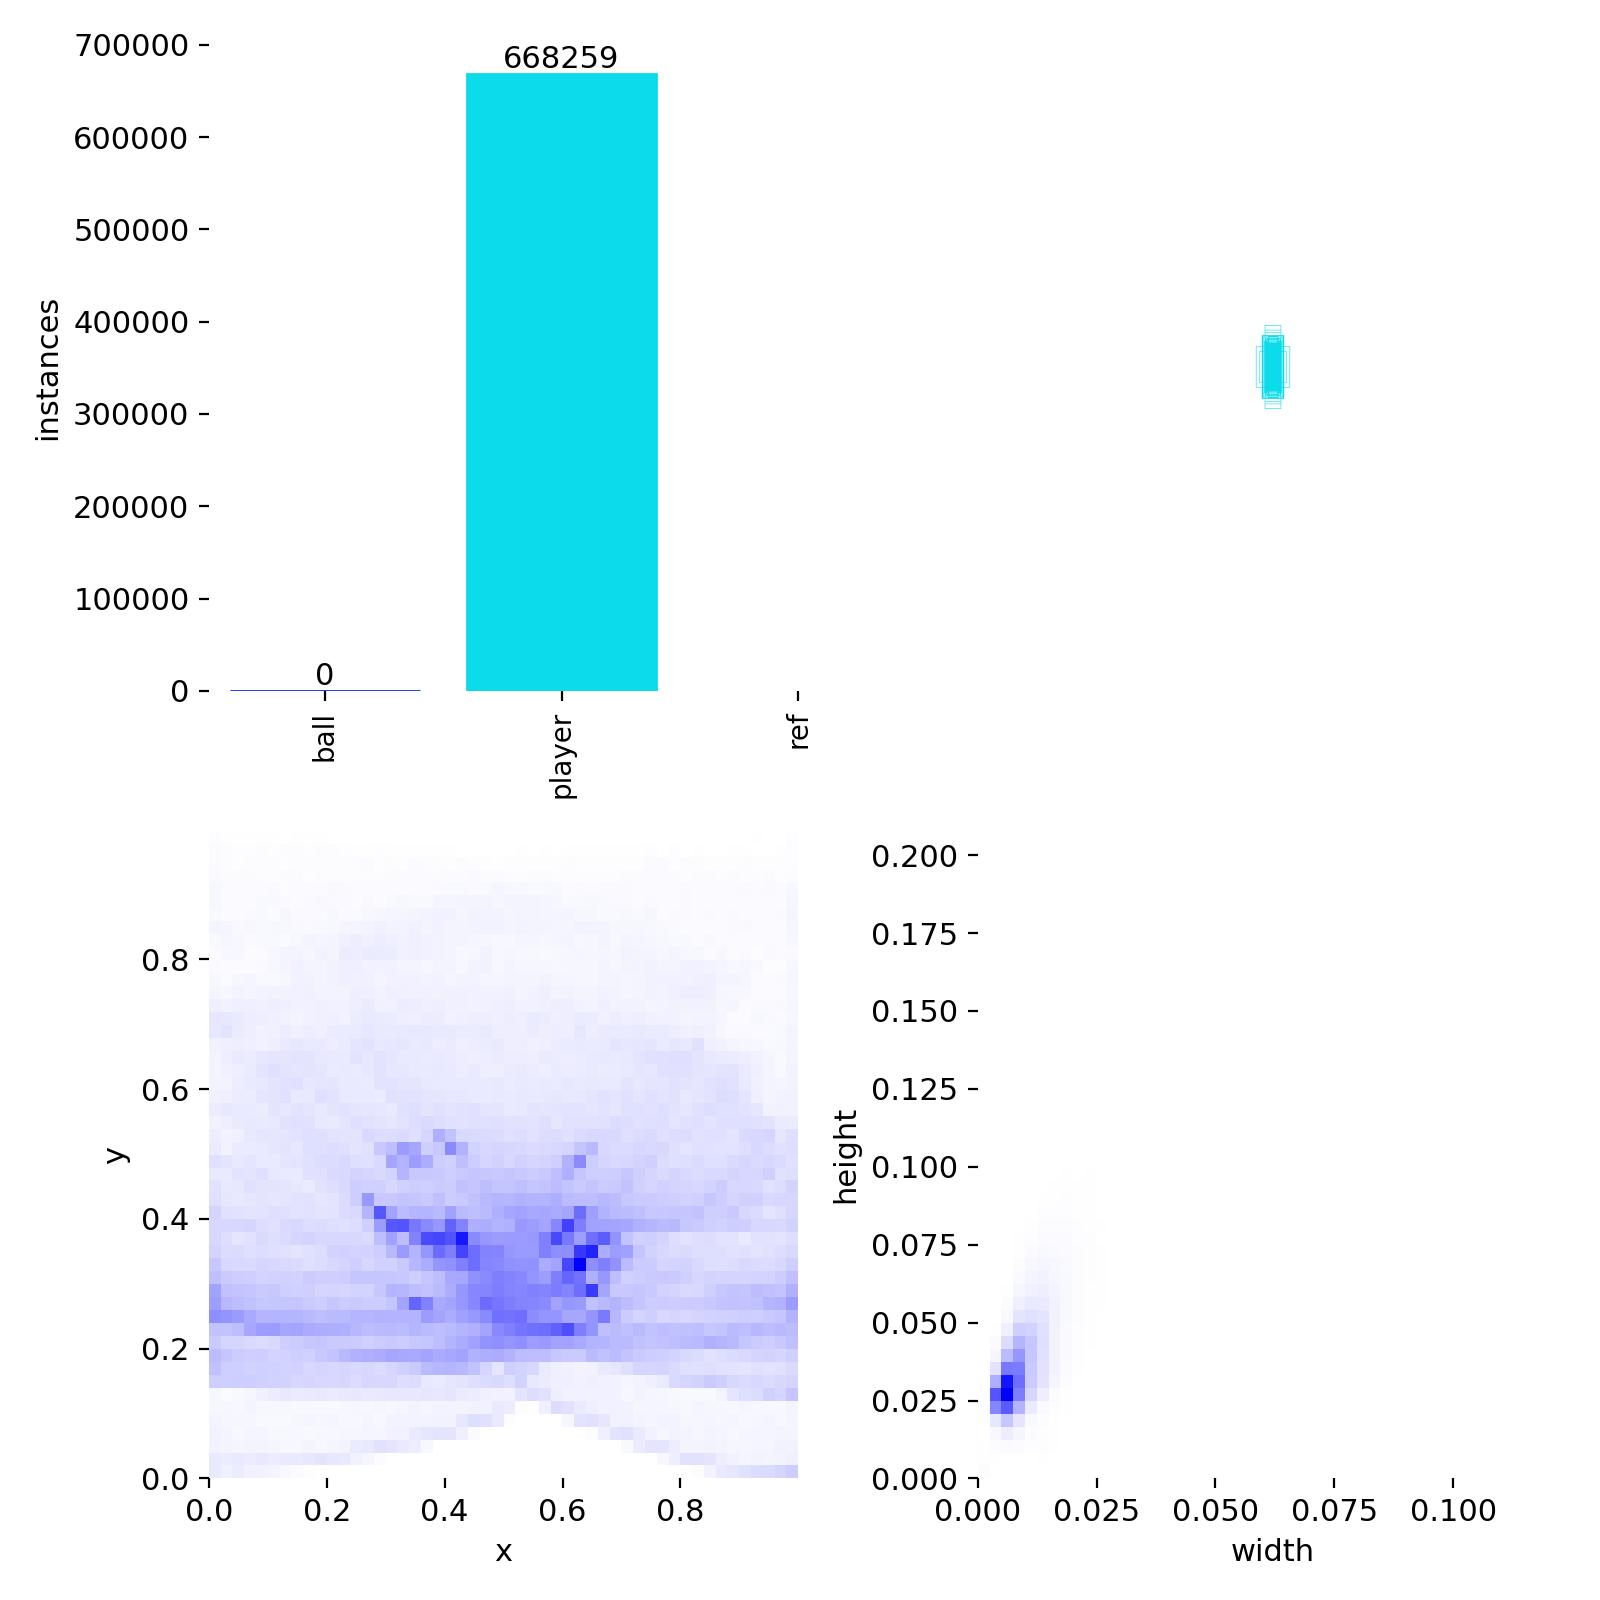
\includegraphics[width=\textwidth]{Imagenes/Propias/labels_sinteticos.jpg}
    \small \textbf{(a)} SoccerSynth-Detection.
\end{minipage}

\vspace{0.4cm}

\begin{minipage}{0.55\textwidth}
    \centering
    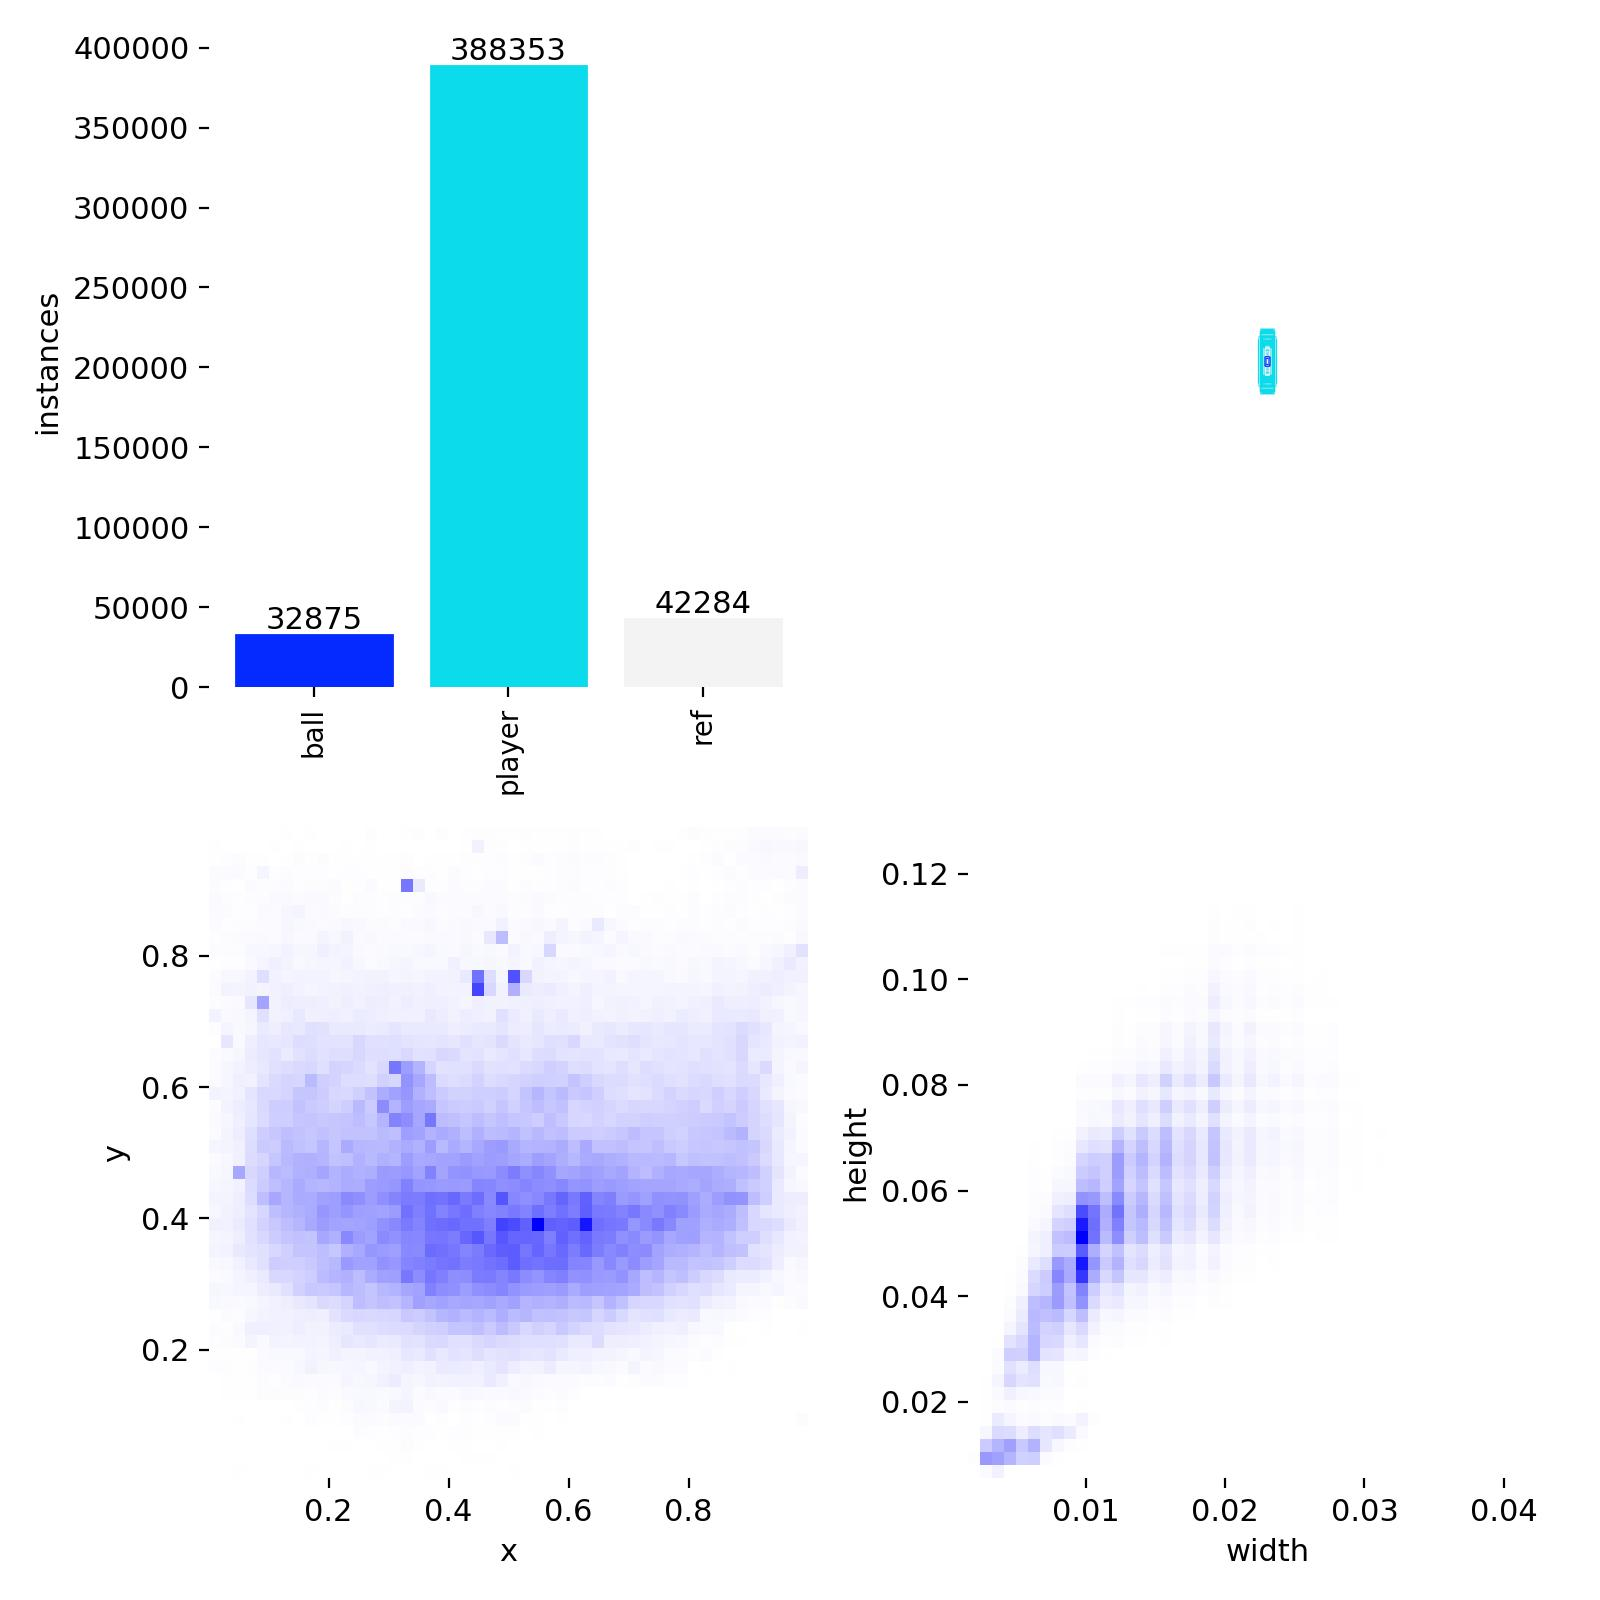
\includegraphics[width=\textwidth]{Imagenes/Propias/labels_dfl.jpg}
    \small \textbf{(b)} Sintéticos + DFL-Bundesliga.
\end{minipage}

\caption[Distribución de etiquetas y cajas en los datasets de fine-tuning]{
Distribución de clases, posiciones normalizadas y tamaños de las cajas delimitadoras en los conjuntos utilizados durante el \textit{fine-tuning} secuencial.
}
\label{fig:datasets_summary}
\end{figure}

Como se aprecia en la \hyperref[fig:datasets_summary]{Figura~\ref*{fig:datasets_summary}}, los datos sintéticos están centrados en la detección de jugadores, mientras que DFL-Bundesliga introduce clases adicionales: balón y árbitro. Por tanto, la segunda fase no solo trabaja sobre imágenes reales, sino también sobre un problema más complejo y desbalanceado. Esto explica que las métricas sean inferiores respecto a la fase sintética sin que ello implique necesariamente un empeoramiento del detector.

La \hyperref[fig:confusion_finetuning_compare]{Figura~\ref*{fig:confusion_finetuning_compare}} muestra las matrices de confusión obtenidas en las dos fases del \textit{fine-tuning} secuencial. En la fase sintética, como ya se había comentado, solo aparece la clase \texttt{player}, con un rendimiento bastante bueno. En la fase DFL-Bundesliga, en cambio, aparecen clases adicionales como \texttt{ball} y \texttt{ref}, lo que permite analizar mejor los errores entre categorías del dominio futbolístico. En particular, se observa que la clase \texttt{player} presenta un comportamiento más estable, mientras que clases menos frecuentes o visualmente más difíciles, como \texttt{ball} y \texttt{ref}, introducen mayor complejidad.

\begin{figure}[H]
\centering

\begin{minipage}{0.55\textwidth}
    \centering
    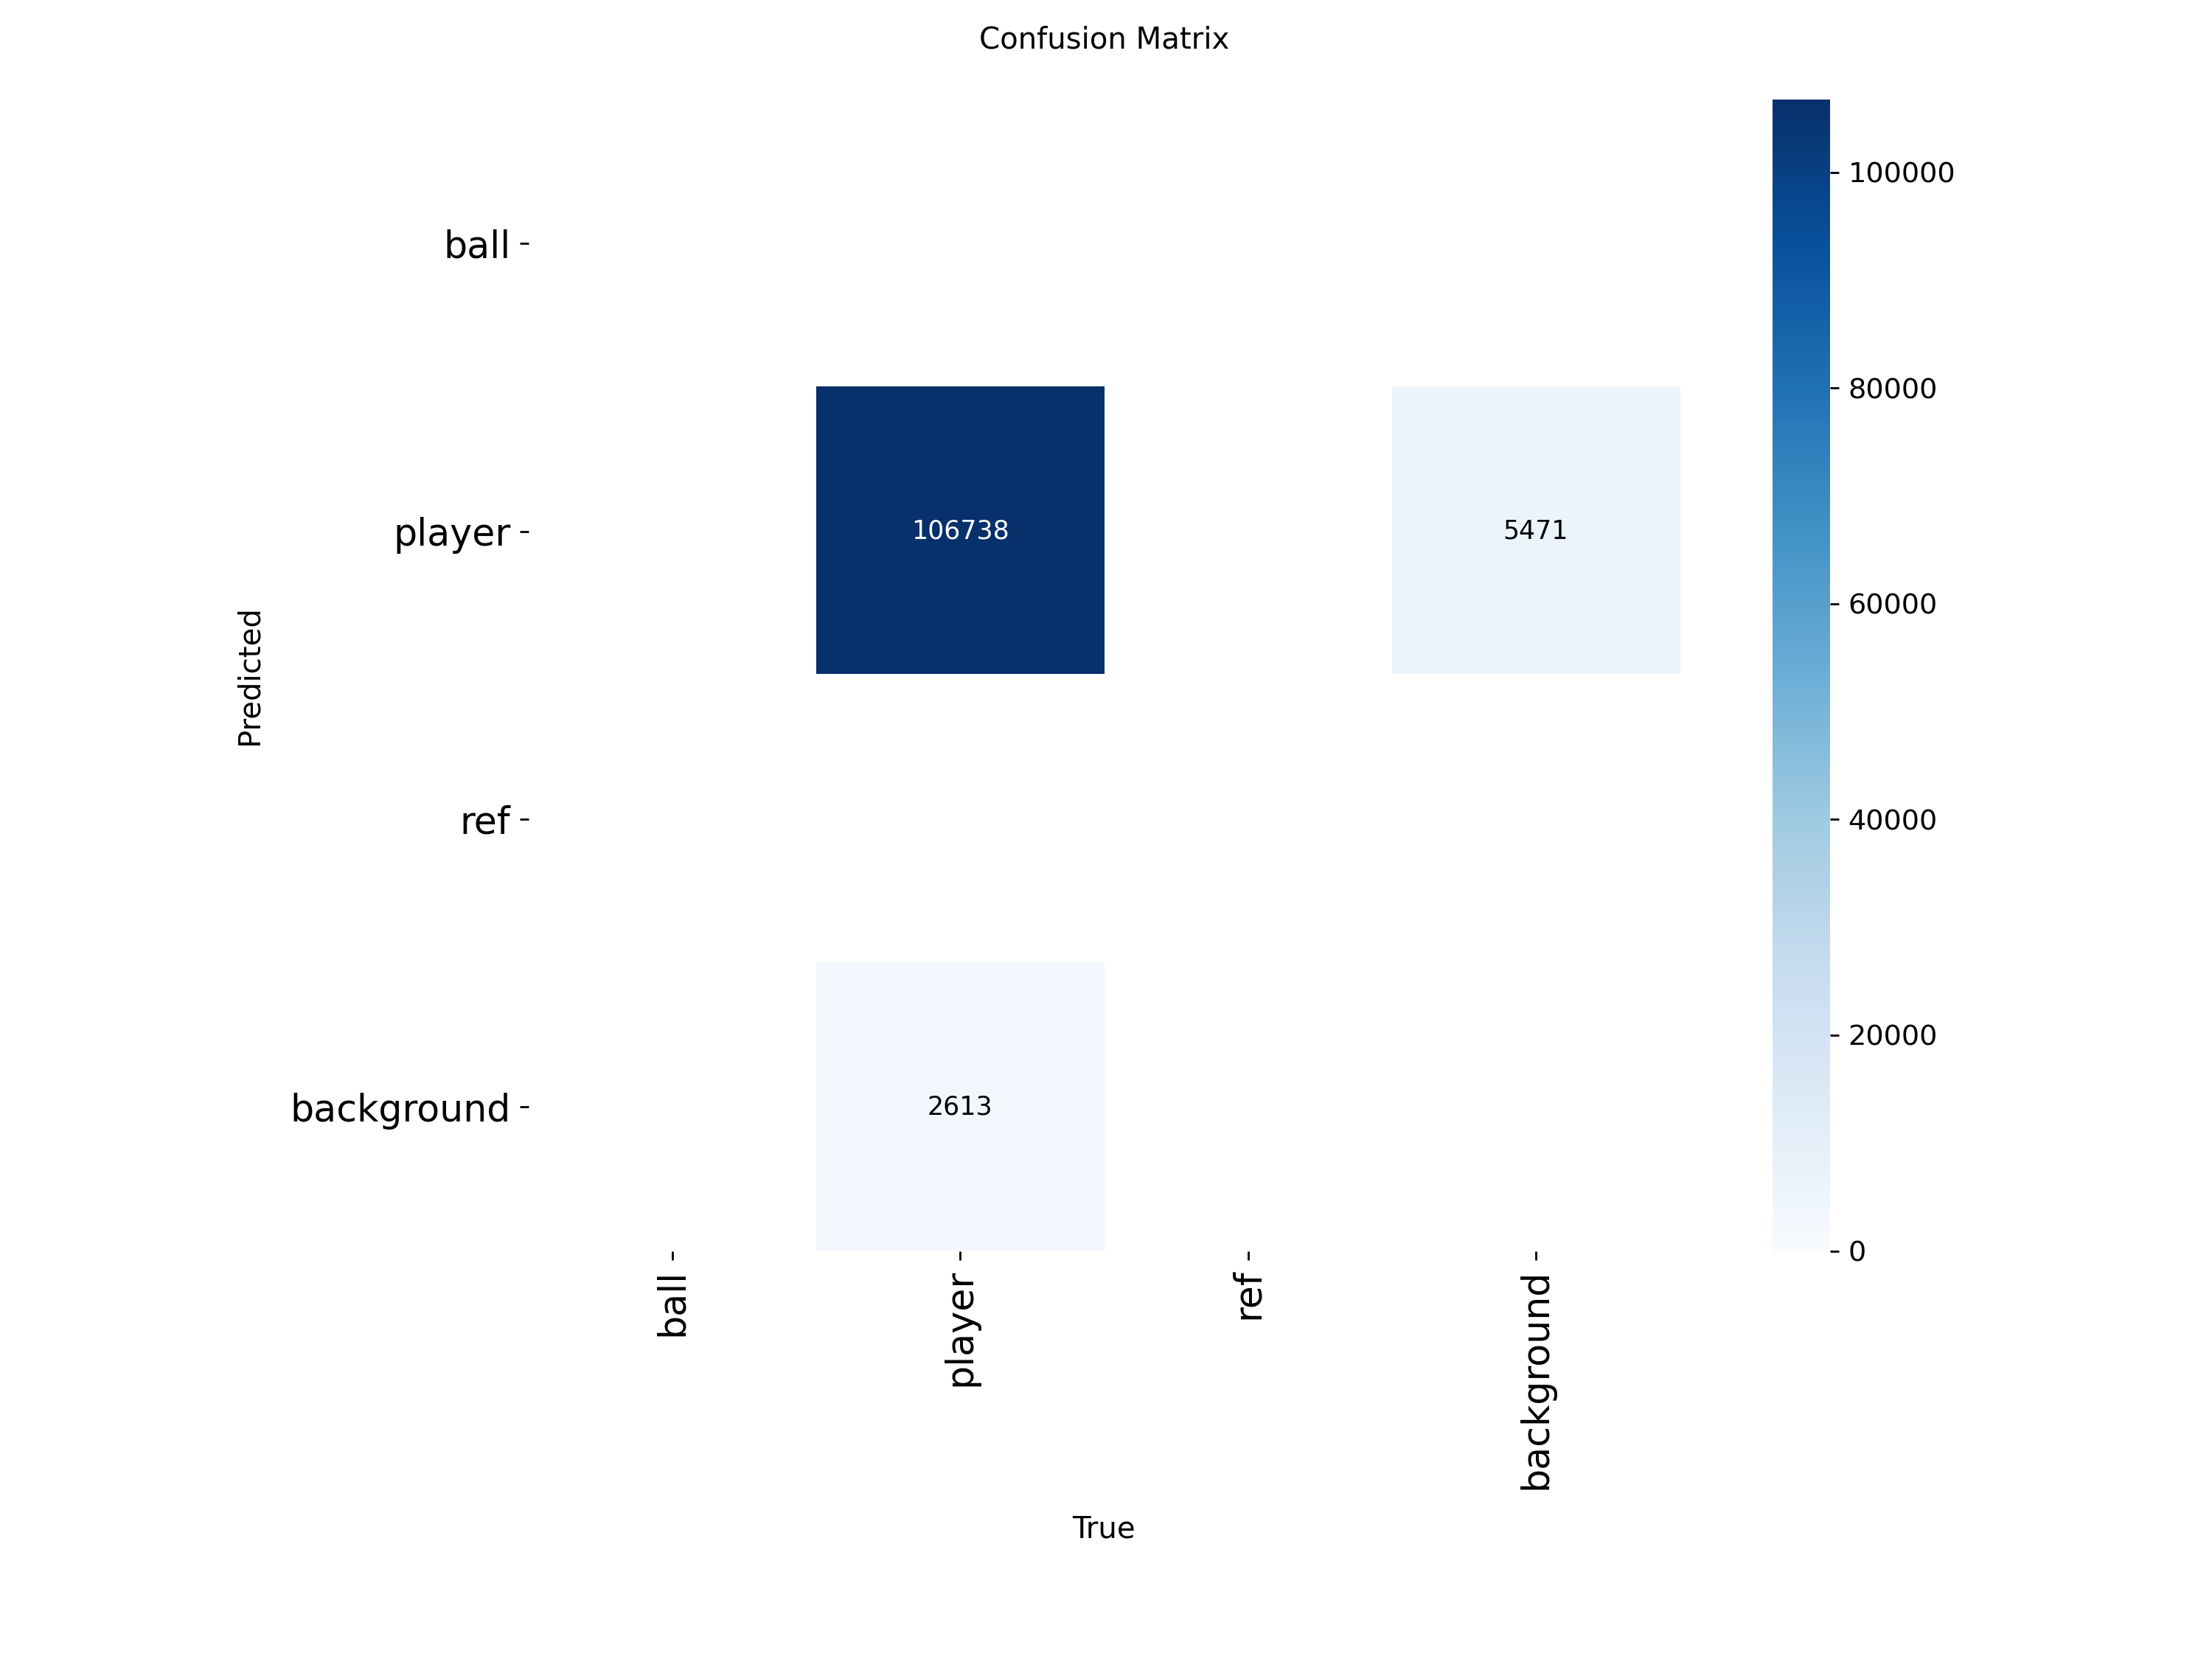
\includegraphics[width=\textwidth]{Imagenes/Propias/confusion_sinteticos.png}
    \small (a) Matriz de confusión en Datos Sintéticos
\end{minipage}

\vspace{0.4cm}

\begin{minipage}{0.55\textwidth}
    \centering
    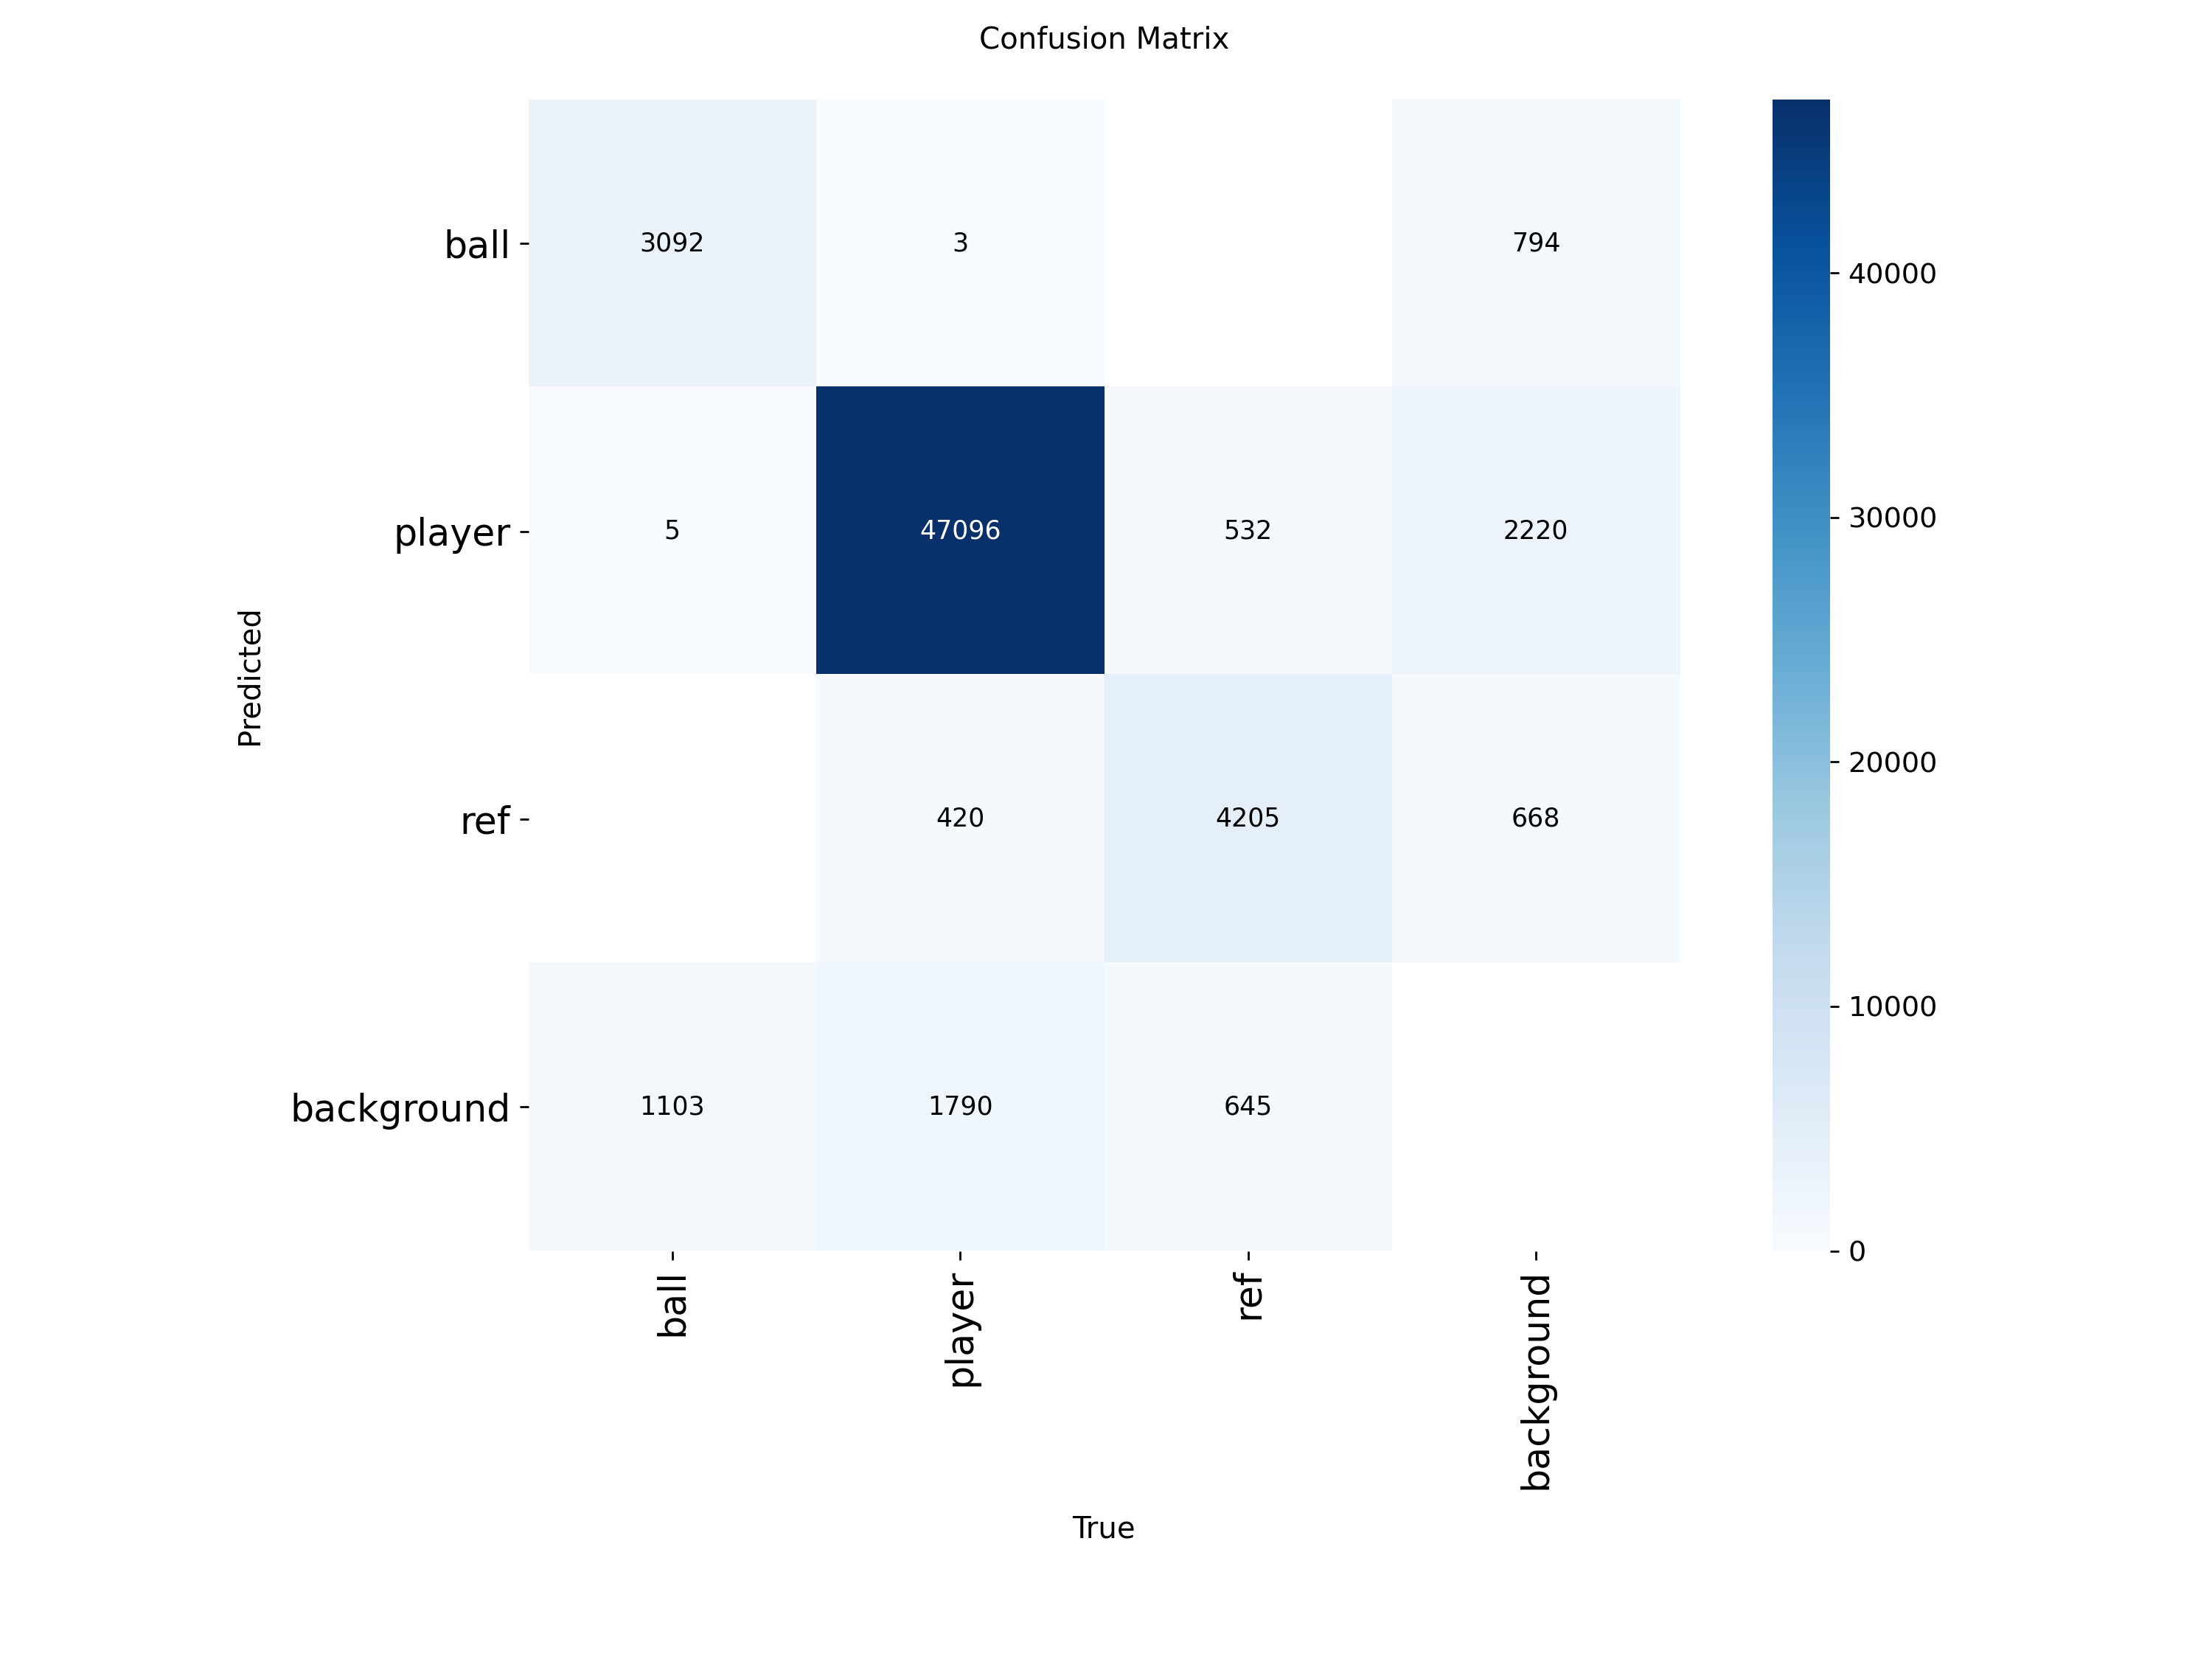
\includegraphics[width=\textwidth]{Imagenes/Propias/confusion_dfl.png}
    \small (b) Matriz de confusión en DFL-Bundesliga.
\end{minipage}

\caption[Matrices de confusión en los datasets de fine-tuning]{
Matrices de confusión en los datasets utilizados durante el \textit{fine-tuning} secuencial. La categoría \texttt{background} no corresponde a una clase entrenada del detector, sino que se incluye en la matriz para representar errores de detección, como objetos reales no detectados o predicciones que no se corresponden con ninguna anotación.
}


\label{fig:confusion_finetuning_compare}
\end{figure}

\subsection{Evaluación sobre la validación de DFL-Bundesliga}

Tras el entrenamiento, se realizó una comparación adicional entre los modelos sobre una misma partición de evaluación: el conjunto de validación de DFL-Bundesliga. El objetivo de esta prueba era comparar ambos detectores bajo un mismo dominio y con las mismas clases de evaluación. Aunque esta partición no se utilizó para actualizar los pesos durante el entrenamiento, no debe interpretarse como un conjunto externo completamente independiente, ya que pertenece al mismo dominio que la segunda fase del \textit{fine-tuning} secuencial.

\subsubsection{Modelos comparados}

En esta evaluación se compararon dos modelos. El primero corresponde al detector afinado directamente sobre el dataset Roboflow fútbol. El segundo corresponde al detector obtenido mediante el proceso secuencial de \textit{fine-tuning}, entrenado primero sobre SoccerSynth-Detection y refinado posteriormente sobre DFL-Bundesliga.

La evaluación se realizó sobre las clases comunes del conjunto de validación: \texttt{ball}, \texttt{player} y \texttt{ref}. La clase \texttt{goalkeeper}, presente en el modelo entrenado con Roboflow fútbol, no se evaluó como categoría independiente, sino que se mapeó a \texttt{player} para mantener una definición de clases común entre ambos modelos.


\subsubsection{Métricas utilizadas}

Las métricas de precisión, recall, F1 e IoU ya se definieron previamente en la \hyperref[subsec:metricas-deteccion-objetos]{Sección~\ref*{subsec:metricas-deteccion-objetos}}. En esta evaluación se utilizan para comparar el comportamiento de los dos detectores sobre la partición de validación de DFL-Bundesliga.

En primer lugar, se analiza el número de instancias reales frente al número de predicciones generadas por cada modelo, como se recoge en la \hyperref[tab:model_comparison_counts]{Tabla~\ref*{tab:model_comparison_counts}}. El número de instancias reales se indica como GT, mientras que el número de predicciones muestra cuántas detecciones produjo cada detector para cada clase. A partir de ambos valores se calcula la tasa de detección, definida como el cociente entre predicciones e instancias reales. Un valor inferior a 1 indica que el modelo tiende a detectar menos objetos de los anotados, mientras que un valor superior a 1 puede indicar mayor cobertura, aunque también riesgo de sobredetección.

La evaluación principal se realiza con un criterio estricto de IoU $\geq 0.50$. Bajo este criterio, una predicción se considera correcta únicamente si la clase coincide con la anotación real y el solape entre ambas cajas supera dicho umbral. A partir de esta correspondencia se calculan precisión, recall y F1 para cada clase, cuyos resultados se muestran en la \hyperref[tab:model_comparison_iou50]{Tabla~\ref*{tab:model_comparison_iou50}}.

Además, se calculan métricas más laxas para analizar la localización aproximada de los objetos, recogidas en la \hyperref[tab:model_comparison_soft]{Tabla~\ref*{tab:model_comparison_soft}}. El recall con IoU $\geq 0.10$ permite comprobar si el modelo detecta el objeto en una zona cercana aunque la caja no encaje con precisión. Esta métrica es útil en fútbol porque algunos objetos, especialmente el balón, pueden detectarse en la zona correcta pero con cajas poco estables. También se incluye un recall basado en centro, que considera correcta una detección si el centro de la caja real cae dentro de alguna caja predicha de la misma clase. Por último, la confianza media resume la seguridad promedio con la que cada modelo emite sus predicciones.


\subsection{Resultados cuantitativos}

La \hyperref[tab:model_comparison_counts]{Tabla~\ref*{tab:model_comparison_counts}} recoge el número de instancias reales y predicciones de cada modelo. La \hyperref[tab:model_comparison_iou50]{Tabla~\ref*{tab:model_comparison_iou50}} muestra la evaluación estricta con IoU $\geq 0.50$, mientras que la \hyperref[tab:model_comparison_soft]{Tabla~\ref*{tab:model_comparison_soft}} incluye métricas más laxas para analizar la localización aproximada de los objetos.

\begin{table}[H]
\centering
\scriptsize
\begin{tabular}{c|c|c|c|c|c}
\textbf{Clase} & \textbf{GT} & \textbf{Pred. Rob.} & \textbf{Pred. Sec.} & \textbf{Tasa Rob.} & \textbf{Tasa Sec.} \\
\hline\hline
\texttt{ball} & 4200 & 1650 & 5111 & 0.3929 & 1.2169 \\
\hline
\texttt{player} & 49570 & 53541 & 51812 & 1.0801 & 1.0452 \\
\hline
\texttt{ref} & 5382 & 5357 & 5503 & 0.9954 & 1.0225 \\
\hline
\end{tabular}
\caption[Instancias y predicciones en la validación de DFL-Bundesliga]{
Número de instancias reales, predicciones y tasa de detección de ambos modelos sobre la partición de validación de DFL-Bundesliga.
}
\label{tab:model_comparison_counts}
\end{table}

\begin{table}[H]
\centering
\scriptsize
\begin{tabular}{c|c|c|c|c|c|c}
\textbf{Clase} & \textbf{Prec. Rob.} & \textbf{Prec. Sec.} & \textbf{Recall Rob.} & \textbf{Recall Sec.} & \textbf{F1 Rob.} & \textbf{F1 Sec.} \\
\hline\hline
\texttt{ball} & 0.6582 & 0.6312 & 0.2586 & 0.7681 & 0.3713 & 0.6929 \\
\hline
\texttt{player} & 0.8642 & 0.9217 & 0.9335 & 0.9633 & 0.8975 & 0.9420 \\
\hline
\texttt{ref} & 0.7000 & 0.8390 & 0.6968 & 0.8579 & 0.6984 & 0.8483 \\
\hline
\end{tabular}
\caption[Comparación estricta con IoU $\geq 0.50$]{
Comparación estricta con IoU $\geq 0.50$ entre el modelo Roboflow y el modelo secuencial SoccerSynth+DFL.
}
\label{tab:model_comparison_iou50}
\end{table}

\begin{table}[H]
\centering
\scriptsize
\renewcommand{\arraystretch}{1.15}
\begin{tabular}{c|c|c|c|c|c|c}
\textbf{Clase} & \textbf{R@0.10 Rob.} & \textbf{R@0.10 Sec.} & \textbf{Centro Rob.} & \textbf{Centro Sec.} & \textbf{Conf. Rob.} & \textbf{Conf. Sec.} \\
\hline\hline
\texttt{ball} & 0.3114 & 0.8340 & 0.3129 & 0.8357 & 0.3522 & 0.5078 \\
\hline
\texttt{player} & 0.9427 & 0.9664 & 0.9743 & 0.9871 & 0.7394 & 0.7942 \\
\hline
\texttt{ref} & 0.7150 & 0.8610 & 0.7179 & 0.8634 & 0.6122 & 0.6951 \\
\hline
\end{tabular}
\caption[Métricas laxas en la validación de DFL-Bundesliga]{
Métricas laxas y confianza media de ambos modelos sobre la partición de validación de DFL-Bundesliga. R@0.10 indica recall con IoU $\geq 0.10$, Centro indica recall basado en centro, Rob. corresponde al modelo entrenado sobre Roboflow fútbol y Sec. al modelo secuencial SoccerSynth+DFL.
}
\label{tab:model_comparison_soft}
\end{table}

\subsection{Interpretación de los Resultados}
Los resultados muestran una mejora clara del modelo secuencial SoccerSynth+DFL sobre la partición de validación de DFL-Bundesliga. La diferencia es especialmente notable en la clase \texttt{ball}: el modelo Roboflow detecta 1650 balones frente a 4200 instancias reales, con un recall estricto de 0.2586, mientras que el modelo secuencial produce 5111 predicciones y alcanza un recall estricto de 0.7681. Aunque su precisión en balón es ligeramente menor, el aumento de cobertura resulta muy relevante para el sistema, ya que el balón es uno de los objetos más pequeños y difíciles de detectar.

En la clase \texttt{player}, el modelo secuencial también mejora las métricas principales, pasando de un F1 de 0.8975 a 0.9420. En la clase \texttt{ref}, la mejora es igualmente consistente, con un aumento del F1 de 0.6984 a 0.8483. Además, las métricas laxas muestran que el modelo secuencial localiza mejor los objetos incluso cuando se relaja el criterio de solape, lo que sugiere una mayor robustez espacial en este dominio.

Estos resultados indican que la estrategia de adaptación con datos sintéticos seguida de refinamiento sobre DFL-Bundesliga es más adecuada para este escenario que el entrenamiento directo sobre el dataset pequeño de Roboflow. No obstante, esta comparación debe interpretarse teniendo en cuenta que se realiza sobre la partición de validación de DFL-Bundesliga, por lo que no constituye una evaluación externa completamente independiente.

La decisión final del detector no debe basarse únicamente en estas métricas de detección aislada. El sistema completo depende también del comportamiento del tracking, de la estabilidad temporal de las identidades y de cómo se comporta el modelo sobre vídeos reales, donde aparecen compresión, movimiento de cámara, cambios de plano y oclusiones. Por este motivo, aunque esta comparación favorece al modelo sintético+DFL, la decisión final se deja abierta hasta completar las pruebas de tracking sobre vídeo real.